\documentclass[11pt]{article}

\usepackage[utf8]{inputenc}
\usepackage[spanish]{babel}
\usepackage{geometry}
\geometry{left=20mm, right=20mm, top=20mm}
\usepackage[dvipsnames]{xcolor}

\usepackage{xurl}  % Allow line breaks at hyphens

\usepackage{hyperref}
\hypersetup{colorlinks=True, urlcolor=RoyalBlue}

\usepackage{graphicx}
\usepackage{float}

\usepackage{verbatim}

\begin{document}

\section*{Pregunta 01: Manejo de relaciones en MongoDB}

MongoDB maneja las relaciones entre documentos mediante dos enfoques principales: embebidos y referenciados. 

\begin{enumerate}
    \item \textbf{Enfoque embebido:} Los datos relacionados se almacenan dentro del mismo documento en forma de subdocumentos o arreglos.
    \begin{itemize}
        \item Ventajas:
        \begin{itemize}
            \item Acceso rápido a la información sin necesidad de realizar un \textit{join}.
            \item Adecuado cuando los datos relacionados se consultan siempre en conjunto.
        \end{itemize}
        \item Desventajas:
        \begin{itemize}
            \item Genera documentos muy grandes y con redundancia si los datos se repiten.
            \item Dificultad de mantenimiento cuando la relación crece demasiado.
        \end{itemize}
    \end{itemize}

    \item \textbf{Enfoque referenciado:} Los documentos se almacenan en colecciones distintas y se enlazan mediante un identificador único (\texttt{ObjectId}).
    \begin{itemize}
        \item Ventajas:
        \begin{itemize}
            \item Más flexible y escalable en aplicaciones de gran tamaño.
            \item Evita la duplicidad de datos y facilita su reutilización.
        \end{itemize}
        \item Desventajas:
        \begin{itemize}
            \item Las consultas pueden requerir múltiples accesos (\textit{join manual}).
            \item Aumenta la complejidad de la lógica en la aplicación.
        \end{itemize}
    \end{itemize}
\end{enumerate}

En comparación con PostgreSQL, este último utiliza claves foráneas que garantizan la integridad referencial de manera nativa, mientras que MongoDB prioriza la flexibilidad y el rendimiento, sacrificando la consistencia estricta de las relaciones.

\vspace{0.3cm}

\section*{Pregunta 02: Ventajas de NoSQL sobre bases de datos relacionales}

Las bases de datos NoSQL, como MongoDB, presentan varias ventajas frente a las bases de datos relacionales tradicionales (RDBMS). Usando como ejemplo una liga deportiva, se destacan los siguientes puntos:

\begin{itemize}
    \item \textbf{Flexibilidad de esquema:} Permite agregar nuevos atributos a jugadores o equipos sin necesidad de modificar una estructura rígida de tablas.
    \item \textbf{Escalabilidad horizontal:} MongoDB puede distribuir los datos entre múltiples servidores mediante \textit{sharding}, mientras que en un RDBMS esto resulta más costoso.
    \item \textbf{Velocidad en operaciones:} Es ideal para registrar resultados en tiempo real de partidos, sin necesidad de transacciones complejas.
    \item \textbf{Representación natural de datos:} Los equipos pueden contener directamente un arreglo de jugadores dentro de su documento, sin requerir múltiples tablas intermedias.
\end{itemize}

En este contexto, NoSQL se adapta mejor a escenarios dinámicos y con alta variabilidad en los datos, como el registro de temporadas, jugadores y estadísticas deportivas.

\section*{Pregunta 03: Creación de base y colección MongoDB}

\begin{figure}[H]
    \centering
    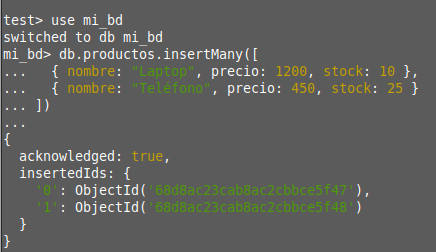
\includegraphics[width=0.8\textwidth]{P03.png}
\end{figure}

Primero se ejecuta el comando \verb'use mi_bd' para seleccionar la base de datos o en su lugar crearla en caso de que no exista y se crea la colección sobre la que se estarán haciendo inserciones de registros.

\section*{Pregunta 04: Consulta MongoDB}

\begin{figure}[H]
    \centering
    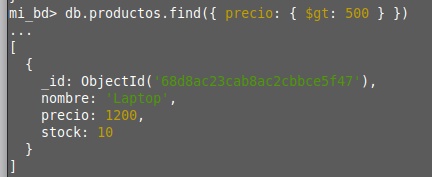
\includegraphics[width=0.8\textwidth]{P04.png}
\end{figure}

Se realiza la consulta sobre la base de datos con el comando \verb'find' sobre la colección creada. En este caso como nos interesa selecionar los valores mayores que 500 se utiliza \verb'$gt' (greater than) para traer los registros que cumplan la condición y el campo sobre el que se desea realizar la consulta (precio).

\section*{Pregunta 05: Actualización y elimincación de registros MongoDB}

\begin{figure}[H]
    \centering
    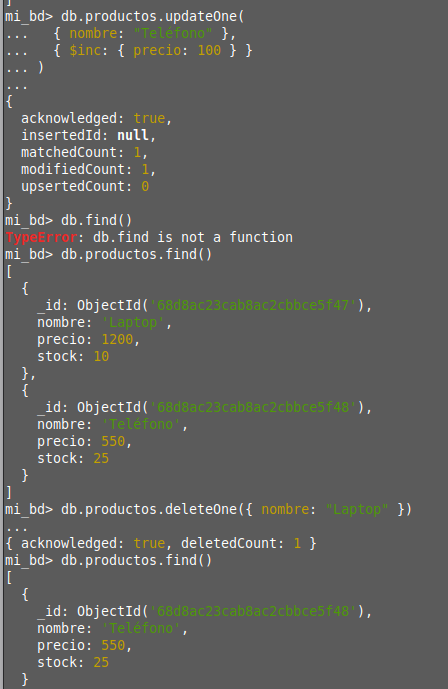
\includegraphics[width=0.4\textwidth]{P05.png}
\end{figure}

Se usa el comando \verb'updateOne' para hacer la actualización de un registros, en este caso deseamos incrementar en 100 el precio de un producto, en nuestro ejemplo sobre el teléfono así que ejecutames \verb'$inc' para indicar el incremento, el aumento que deseamos (100), el campo sobre el cual hacer la actualización (precio) y el producto (teléfono). Posterior, validamos que se haya actualizado el registro con el comando \verb'find', se elimina un valor, en este caso Laptop y para ello se utiliza \verb'deleteOne' y nuevamente con \verb'find' validamos los cambios.

\section*{Referencias}

\begin{enumerate}
    \item Chodorow, K. (2013). \textit{MongoDB: The Definitive Guide}. O’Reilly Media. 
    \item MongoDB Inc. (2023). \textit{Data Modeling Concepts}. Recuperado de: \url{https://www.mongodb.com/docs/manual/core/data-modeling-introduction/}
    \item MongoDB Inc. (2023). \textit{CRUD Operations}. Recuperado de: \url{https://www.mongodb.com/docs/manual/crud/}
    \item Stonebraker, M., \& Hellerstein, J. M. (2015). \textit{What Goes Around Comes Around}. Communications of the ACM, 58(7), 10–13. 
    \item Silberschatz, A., Korth, H., \& Sudarshan, S. (2019). \textit{Database System Concepts} (7th ed.). McGraw-Hill.
\end{enumerate}

\end{document}